%************************************************
\chapter{Implementation}\label{ch:implementation}
%************************************************

\begin{itemize}

\item{
	Intro text describing what is implemented, features, hardware
}
\item{
	Show user interface and describe mechanics. how to speech and gesture. mention activation angle study and show plot. 
}
\item{
	Mention Modules and communicationManager. show communication protocol. maybe uml diagram of whole application
}
\item{
	Describe Handheld module. introduce spotify api + webapi wrapper.
}
\item{
	Describe Wear module
}
\item{
	possible improvements and restrictions to the program (like leaving out unneeded spotify features), input feedback
}

\end{itemize}

This chapter describes the smartwatch controlled mobile music player implementation. It gives an insight into the chosen interaction techniques, the mobile-wear communication and the core music player functions.

The essential music library is provided by a private Spotify\footnote{Music streaming service: \url{www.spotify.com}} premium account. The prototype is divided into two separate applications, i.e. mobile (handheld) and wear (smartwatch). Users are able to access all features of the mobile application via the smartwatch application. In order to make use of the focused-casual continuum \cite{pohl2013focused}, three interaction techniques, differing in the amount of control granted, are available for the user:
\begin{itemize}
\item{Touch}
\item{Speech}
\item{Gesture}
\end{itemize}
Each technique can be used for the simpler actions of the music player such as play and pause, skip to previous or next song and changing the volume. However, for the more complex interactions, e.g. choosing a playlist, only the touch and speech interaction methods suffice. Gesture and speech input can be performed casually while not even looking at the device (the smartwatch). The following section describes the functionality and the power of the different methods.

Both applications are implemented for the android platform. The handheld device has no further hardware or software requirements other than supporting the android wearable \ac{API} so a Samsung Galaxy S6 is chosen. The smartwatch application certainly requires the device to be equipped with a acceleration sensor and a microphone. A moto360 from Motorola is well suited for this. Both devices need to support Bluetooth, too.

\section{User Interface}
The \ac{GUI} from the mobile application only differs in appearance from the wear \ac{GUI}. In terms of control over the music player, both versions offer the same possibilities and show the same information at any given time. The wear application, however, additionally introduces speech and gesture interactions which the mobile application is not capable of.

\subsection{Touch Input - \ac{GUI}}
Both \ac{GUI}s are designed to be simple and straightforward. The mobile version mainly consists of two areas. Figure \ref{fig:mobileGUI} depicts a screenshot of this layout. A control panel is situated at the bottom of the screen. Above this is a left-right scrollable pager containing different kinds of lists. \marginpar{Categories are Spotify's extended version of genres} The scrollable list pager contains five lists, one for each music arrangement which are playlists, songs, albums, artists and categories.
\begin{figure}[bth]
	\myfloatalign
	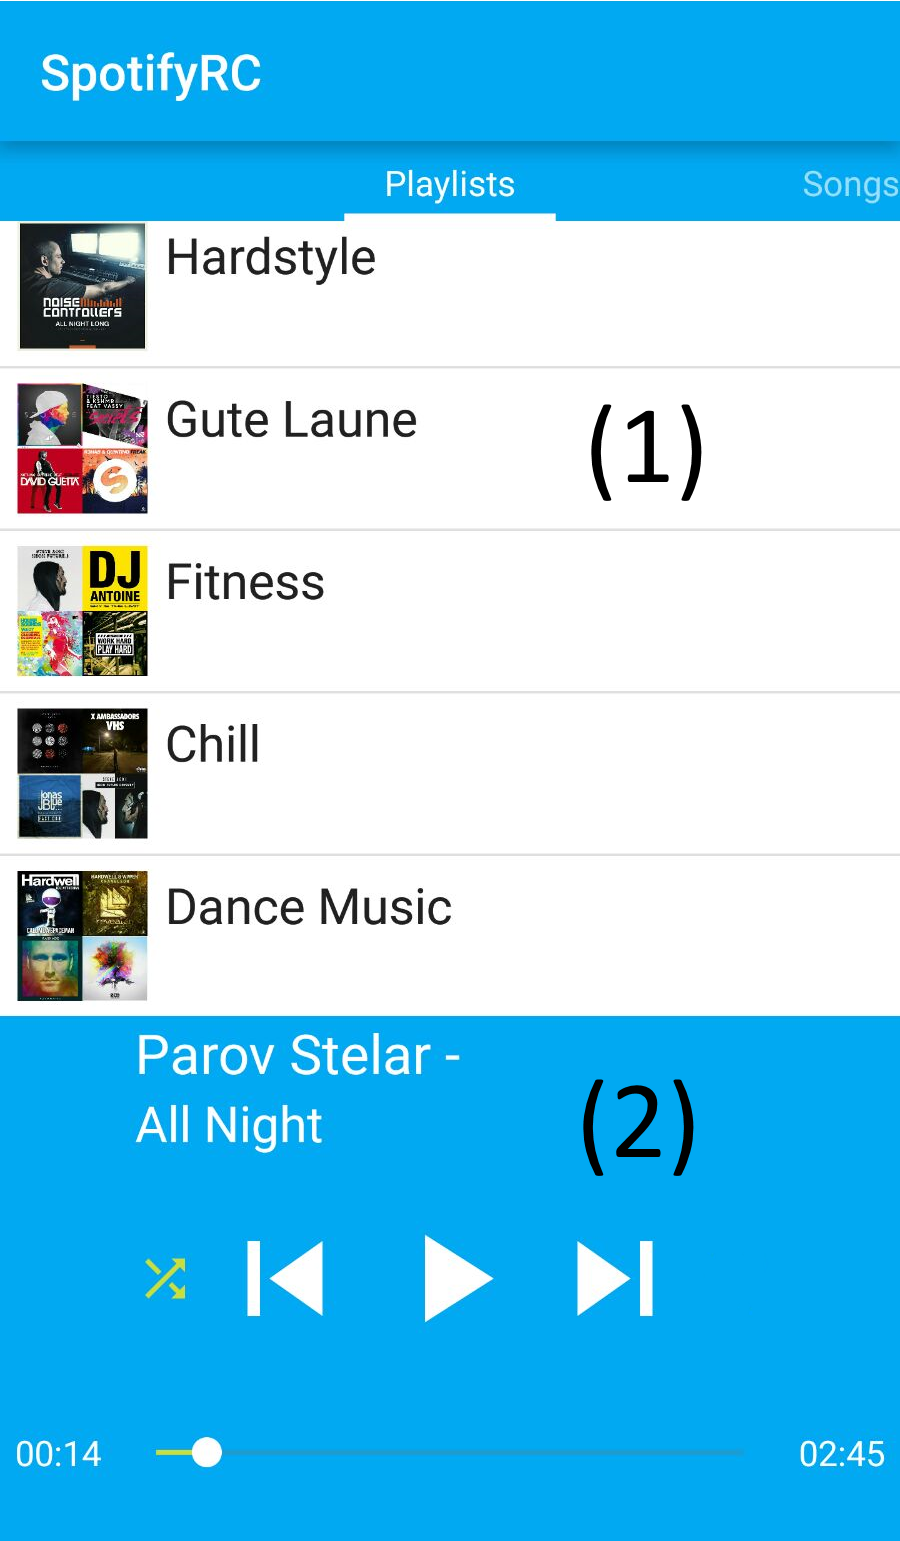
\includegraphics[width=.45\linewidth]{img/mobileGUIlabeled.png}
	\caption{\ac{GUI} of the mobile application. (1) shows the left-right scrollable list pager with indicators which list is shown at the top. (2) shows the player control panel in blue.}
	\label{fig:mobileGUI}
\end{figure}

The control panel located beneath the list pager contains four control buttons such as a shuffle button including on-off indicator, a skip to previous song button, a play-pause button and a skip to next button. Information on the name of the current song and artist can be found above these buttons. The track's progress and total duration can be found at the very bottom of the screen.

%TODO gui watch: take screenshots from watch app

\subsection{Speech Control}

\subsection{Gesture Control}

%Chapter \ref{ch:implementation} 


%*****************************************
%*****************************************
%*****************************************
%*****************************************
%*****************************************




